% ---------------------------- comment out when compiling the full document -------------------
\documentclass[12pt]{mytustyle}  % default square logo 
\usepackage{amssymb}
\usepackage{caption}
\usepackage{upgreek}
\usepackage{subfig}

\usepackage{packages/fancyhdr}% http://ctan.org/pkg/fancyhdr
\pagestyle{fancy}% Change page style to fancy
\fancyhead[OR]{\renewcommand\thesection}
\fancyhead[ER]{\renewcommand\chaptername}

%\fancyhf{}% Clear header/footer
%\fancyhead{}
%\fancyhead[RO, LE]{Current monitoring}
%\fancyfoot{}
%\fancyfoot[RO, LE]{\thepage}% \fancyfoot[R]{\thepage}
\renewcommand{\headrulewidth}{0.7pt}% Default \headrulewidth is 0.4pt
%\renewcommand{\footrulewidth}{0.7pt}% Default \footrulewidth is 0pt
%\rfoot{\thepage}
\usepackage{enumitem}
\setlist[description]{leftmargin=0cm,labelindent=0cm}


\begin{document}
\baselineskip=15pt
% ---------------------------------------------------------------------------------------------------------------



% ---------------------------------------------------------------------------------------------------------------
\chapter{Current monitoring}
% ---------------------------------------------------------------------------------------------------------------
	- Real-time particle identification
		- Pulse shape (width, area. . .) and its constraints
		- Device constraints

Diamond sensors have a very fast signal response due to their low capacitance. The electrical signal created by drifting charge carriers retains its shape without significant distortion. When the sensor is used together with a fast current amplifier with a high broadband limit ($\sim$2~GHz) and a readout device with a similar limit, the information about the drifting charges is retained. For instance, a proton creates the free e-h pairs along its trajectory. The electrons and holes start drifting immediately. Those closest to the electrodes recombine quickly whereas those at the opposite side contribute to the induced signal for longer. The resulting signal is therefore a triangular pulse with a steep rising edge and a gentle falling edge. This means that it is possible to determine, with a certain probability, the type of radiation detected by the diamond sensor. Furthermore, it is possible to determine the speed of the charge carriers, as was done in chapter~\ref{}. This, however, only applies to sCVD diamond . Its uniform carbon lattice allows the ionisation profiles to retain their shape, unlike in pCVD material, laden with grain boundaries, or in even in silicon where the shape is deformed due to p-n junction non-uniformities.

Chapter~\ref{} shows that the shape is heavily dependent on several factors, such as environmental temperature and received irradiation dose. At temperatures lower than 150~K the signal from an $\upalpha$ starts deteriorating due to recombination of charges in the charge cloud. Sensor irradiation, on the other hand, introduces charge traps, which cause the signal to decay exponentially. These two factors are a significant limitation for particle identification. Priming can improve the charge collection and longterm stability of the pulse shapes. To improve the measurement further, a high bias voltage has to be applied, with the right polarity for hole collection. These settings will yield a high and narrow $\upalpha$ pulse, increasing the measurement SNR. 


%The most straightforward way is to discriminate between $\upalpha$ (rectangular) and $\upgamma$ or proton (triangular) pulses.

\begin{center}
\begin{tabular}{l*{1}{c}}
Factor              & Operating range \\
\hline
Sensor material & sCVD diamond \\
Sensor thickness & $500~\mu m$ \\
Temperature & 150~K -- 400~K \\
Radiation dose & $1\times10^{13}~neq~cm^{-2} s^{-1}$ \\
Charge carriers & holes \\
Bias voltage & $\sim1~V \mu m^{-1}$ \\
Signal-to-noise & 5 \\
\end{tabular}
\captionof{table}{Limitations to particle identification}
\label{tab:limits}
\end{center}




This chapter describes an application that carries out particle identification using pulse shape analysis. It was developed to count neutrons emitted by a neutron reactor. In this case the device has to be able to filter out the photon background with a rate several orders of magnitude higher than the neutron rate. Overall detected rate in a neutron reactor can easily exceed $10^8$ particles $cm^{-2}s^{-1}$, depending on the distance of the detector from the reactor core. The device has to be able to cope with such high rates. It also needs to be dead time free or at least close to that, to minimise the counting error. At these rates, it still has to be able to identify the types of pulse. This type of online analysis cannot be done in software. It has to be implemented in an FPGA.







%To sum up, observing the ionisation profiles in sCVD diamond allows us to determine the type of radiation. 



%- pulse shape
%- constraints
%- single






% ---------------------------------------------------------------------------------------------------------------
%\clearpage
\section{Real-time particle identification}
\label{sec:rtpi}
% ---------------------------------------------------------------------------------------------------------------
Pulse shape analysis (PSA) is a common software tool for analysing sensor response to impinging particles. It is usually done using software that runs over big amounts of data that have been acquired and saved to storage. This offline analysis can be repeated and improved. However, the saved data take up a lot of storage space. In addition, saving raw waveform data requires a system capable of a high data throughput and fast data storing. For instance, an oscilloscope can save up to 100~waveforms per second. This means that there is a high measurement dead time. To avoid the high dead times, the software algorithms can be ported to the FPGA where they analyse the incoming signal in real time. The signal is then discarded and only the analysis results are saved, decreasing the storage space significantly.

The offline pulse shape analysis has already been used for particle identification with a diamond sensor. An effort has been made to implement an online and real time application for this analysis by porting the algorithms into an FPGA. This section first describes the device specifications Then it describes in detail the PSA algorithms and the structure of the code. Finally it discusses the performance results.



\section{Device specifications and constraints}
The ROSY box has a single BNC input with the termination $50~\Omega$ or $1~M\Omega$ with a DC or AC coupling. The analog chain has a 250~MHz bandwidth limit. The input range can be set from $\pm$50~mV up to $\pm$5~V. The signal offset can be set to any value within this range. The ADC is samples this signal with an 8-bit precision at a rate of up to 5~GSPS. The PSA uses the highest sampling to achieve width measurement resolution of 0.2~ns. The spectroscopic application does not need such a fine timing resolution and therefore operates at a reduced sampling rate of 0.8~ns. The amplitude resolution depends on the chosen input range, but at 256 ADC counts per sample, it can be as low as 0.39~mV~s$^{-1}$ at the range of $\pm$50~mV and as high as 39~mV~s$^{-1}$ at the range of $\pm$5~V.

The logic structure of the PSA is designed using VHDL and runs on Xilinx Virtex~5. The PSA is capable of a maximum counting rate of $1.56\times10^8$ pulses per second, yielding a 6.4~ns double pulse resolution. The analysis is more time consuming; the maximum throughput rate of the pulse shape analysis is $\sim10^7$ pulses per second. This means that after every pulse, the device has a dead time of approximately 100$\pm$15~ns, depending on the width of the pulse being analysed. Any pulse arriving during the analysis of the previous one will be counted, but not analysed. Any two pulses with the distance between the rising edges lower than 6.4~ns will be counted as a single pulse.

The device is very sensitive to noise pick-up. Therefore the setup must be designed to minimise the pick-up by means of proper shielding, use of high-quality cables etc. The relatively low bandwidth limit filters out some high-frequency noise, but not the ringing or higher noise spikes. That is the task for the PSA.

\section{Pulse parameters}
A signal pulse on the input is parametrised during the analysis process. The PSA measures its amplitude, area, width and the slope of its falling edge. The amplitude is the difference between the baseline and the highest sample in the pulse and is given in ADC counts as an 8-bit value. The area is defined as the sum of amplitudes of all samples between two defined boundaries within the pulse. The width is defined as the number of samples with a value higher than a set amplitude threshold. If the threshold is at half the maximum amplitude, the resulting width is \emph{full width at half maximum} (FWHM). The falling slope is the maximum negative difference between values of two samples and is given in ADC counts per sample. These parameters can also be used as \emph{qualifiers} for accepting or discarding a pulse. All four parameters limited by the low and high limit are called a \emph{qualifier set}. For instance, a rectangular pulse by an $\upalpha$ particle will always have the same FWHM and a very steep slope. In comparison, a photon will have a lower falling slope value and a narrower FWHM. Therefore the low and high cut on these two qualifiers will make possible to discriminate between the two pulses. Another qualifier is a \emph{form factor} and is defined as the multiplication of measured amplitude and width. This qualifier is then compared to the measured area.


%Every parameter set is saved into a histogram after analysis.  The falling slope is not even a physical quantity, but as will be shown later, can improve the identification. 


%\subsection{Real-time pulse shape analysis algorithm}
\clearpage
\section{Applications}
\label{sec:applications}

The FPGA firmware is designed for systems instrumented with CIVIDEC amplifiers and CIVIDEC sVCD diamond detectors. Three applications are available: \emph{Spectroscopy}, \emph{Pulse Shape Analysis} and \emph{Counter}, each optimised for a specific task. Their capabilities are described below. The firmware runs in ROSY, a readout system by CIVIDEC.

\begin{description}
\item[Spectroscopy] is a tool for measuring energy spectra of radioactive sources. It is used in combination with the CIVIDEC Cx spectroscopic charge amplifier. The signal from the charge amplifier is analysed in real time. The FPGA measures the maximum amplitude of the signal. The amplitude value is ready at the end of the pulse and is stored in the amplitude histogram. Immediately after, the analysis is reset and the system is ready for a new acquisition. Upon request from the software, the histogram is read out, during which the analysis is paused. In addition to the histogram building, the firmware can also store raw pulse waveforms, which can be then read out by the software. The maximum allowed throughput is 1~million counts per second.

\item[Pulse Shape Analysis] is a tool for measuring energy spectra of radioactive sources, with an additional feature. It can identify the type of radiation detected by the diamond detector. By means of the radiation identification, it can subtract the background radiation and only measure the signals from the defined radiation source. It is used in combination with the CIVIDEC C2 fast current amplifier. The firmware receives a current pulse from the detector and digitises it. The pulse is then analysed and parametrised. The analysis module measures its maximum amplitude, full width at half maximum (FWHM), baseline amplitude, falling slope and its area. Then it compares the obtained pulse parameters with the qualifiers set by the software and determines what type of radiation hit the diamond detector. Depending on the qualifiers, the pulse can either be \emph{accepted} or \emph{rejected}. The firmware then stores the parameters of the analysed pulse into histograms. Two histograms exist for each parameter: one for all pulses and one for accepted pulses. In addition, there is one 2D histogram (a scatter plot), which can plot two parameters one with respect to the other. Upon request from the software, all histograms are read out, during which the analysis is paused. The maximum allowed throughput is 1~million counts per second.

\item[Counter] is a tool that measures the count rate and the mean time during counts. It is used in combination with the CIVIDEC Cx, C6 or C2 amplifier. It has one histogram which holds the information about the mean time during counts. The counter is only paused during the readout of the histogram.
 
\end{description}



\section{Description of the firmware}
The applications are built on top of the Picotech framework. The base code handles the communication between the software and the hardware. Furthermore, it provides the interface to the ADC data, the input/output registers and the USB data transfer. The applications have a set of modules that handle the data input and output and a module for signal analysis. The data handling modules are very similar in all the applications to ensure compatibility of the communication between software and firmware and the readout data format. The analysis module, however, is different from one application to the other. 

The data handling layer consists of the final state machine (FSM), the histogram builder, the raw signal handler, the USB FIFO buffer and the register array (see figure~\ref{fig:application}). 


\begin{figure}[!t]
\centering
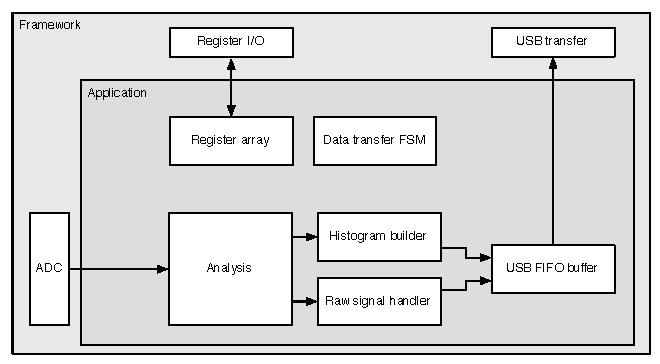
\includegraphics[width=0.9\textwidth]{plots/application}
\caption{Firmware design structure}
\label{fig:application}
\end{figure}


%=====================================================
\subsection{Analysis module}
\label{subsec:algorithm}
This module is different for different applications. The Pulse Shape Analysis (PSA) application has the most complex module design. The spectroscopy application only uses a small part of the PSA design and the Counter application an even smaller one.

The firmware for the PSA module is written entirely in VHDL. The diagram in figure~\ref{fig:architecture} shows the module architecture. The ADC provides the module with 32 digitised signal samples every clock cycle. The signal is routed directly to the pulse analyser and into raw signal handler. The analyser outputs are connected to the I/O registers and to histogram buffers. Both the histogram buffers and raw signal buffers are connected to the USB fifo through a multiplexor. The firmware communication to the controller is done via input/output (I/O) registers (control and status registers, counters) and serially via USB (histogram data, waveforms). 

%\begin{figure}[!ht]
%\centering
%\includegraphics[width=0.9\textwidth]{plots/fpga-arch-ts}
%\caption{Code design plan}
%\label{fig:architecture}
%\end{figure}

The analysis (or parametrisation) is carried out in several steps. The triggering block starts the readout upon signal threshold crossing. The maximum slope of the falling edge is observed. The Amplitude block calculates the pulse height and retains the maximum amplitude while pushing the signal into the pulse buffer. Then the whole pulse is clocked out of the buffer while its FWHM, baseline width and area are measured. Finally, the Form factor is calculated. At the end the Evaluation block takes in all the parametrised information and classifies the pulse according to user-defined cuts. 

%Figure~\ref{fig:pulseana} shows the timing of the data flow within the block. All submodules are described in detail in the following subsections. The waveform in figure~\ref{fig:waveform1} is a simplified representation of the pulse analysis process. The logic bits show which modules within the PSA are active at which stage of the analysis.
\begin{description}
\item[Triggering] module handles signal polarity swapping, triggering on threshold and defining the trigger window. The real-time processing algorithm allows for positive and inverted input signal. However, the PSA only handles positive-polarity pulses. Therefore a negative signal is swapped in the \textit{triggering} block. Signal analysis and readout are then triggered when the signal crosses a user-defined threshold. In addition, the signal has to be over the threshold for a defined number of samples. This is to avoid triggering on noise spikes.
A double clock cycle delay is used on the signal to make sure that the recorded signal window will include the rising edge of the pulse as well as some baseline before it (see figure~\ref{fig:triggerwin}). A \textit{trigger active} signal marks a window that contains the whole pulse including some baseline signal before and after it. 
The trigger can be vetoed by three signals: if the pulse analysis is still taking place, if the input signal exceeds the maximum voltage range or if the data transfer FSM is pausing the analysis due to data transfer.

%\subsubsection{Baseline producer}
%\label{subsub:base}
%This module has two functionalities. It carries out baseline noise filtering and it produces a baseline signal during a pulse. The filtering is implemented as a moving average of four data points. User can choose which four points to use: every first, second, third or fourth sample.
%
%Baseline signal during a pulse is used to calculate pulse height. It is produced by re-playing the last 64 data points of the baseline in a loop (an example shown in figure~\ref{fig:pulsepars}). It is implemented as a double register which replaces the real signal during the trigger window.


\item[Amplitude] block calculates the pulse height from the difference between the pulse and the baseline. It also finds the position of the maximum amplitude within the clock cycle. As stated in section~\ref{subsec:hardware}, the ADC sends 32 8-bit samples every clock cycle. Time delays in the logic prevent it to find the maximum value of the 32 samples within one clock cycle (6.4~ns). Therefore the decision logic has been pipelined in three stages (see figure~\ref{fig:maxval}), which means that the final maximum value is ready three clock cycles after the end of pulse.
\item[Pulse buffer] is a FIFO that stores the signal while its amplitude is being measured. At the end of the pulse the FIFO is read out so that the remaining measurements can take place. 

\item[FWHM] block uses the maximum amplitude to determine the \emph{half-maximum} and to measure the width. To do so, it counts the samples that are above the half-maximum amplitude. However, this method might also count high enough noise spikes before or after the pulse. Hence an improved method, which ``cleans'' the measurement of unintentional additional noise, has been implemented. It is described in section~\ref{sec:vecclean}.
\item[Baseline width] block is the same as the FWHM block, but it measures the width either at 50~\%, 25~\%, 12.5~\% or 6.25~\%, depending on the setting in the register. It also makes use of the special method to avoid overestimations due to including noise in the measurement.
\item[Area] block measures the pulse area by summing up the amplitude values of the samples in the pulse. The boundaries of the summation are defined with the crossing of the amplitude above a certain threshold. Only the samples between those boundaries are summed up. The boundaries can be set at  50~\%, 25~\%, 12.5~\% or 6.25~\% of the maximum amplitude of the pulse. The area measurement makes use of the same routine as the FWHM and Baseline width block to remove the potential outlying samples.

\item[Falling slope] block measures the highest negative difference between amplitudes of two adjacent samples, thus getting the maximum negative slope of the pulse. It is an experimental routine,
\item[Form factor] block is used as a special qualifier for particle identification. It compares the weighted measured area of the pulse with its weighted calculated ``form'', which is defined as the multiplication of the measured amplitude and baseline width. The equation is as follows:
\begin{equation}
\label{eq:formfactor1}
x\cdot a - y \cdot A \cdot BW \geq 0,
\end{equation}
where $a$ is the measured area, $A$ is the amplitude, $BW$ is the baseline width and $x$ and $y$ the weighting factors for the measured and calculated area, respectively. The output of the block is the boolean result of this equation.
\item[Evaluation] block takes in all 

\end{description}


\subsection{Vector cleaning for area and width measurements}
\label{sec:vecclean}
The routine for measuring pulse area and width was designed to improve the measurements with respect to the previous implementation. The core difference is that the new routine precisely defines the edges of a pulse. It does so by means of \emph{vector cleaning}, presented in figure~\ref{fig:samplepulse}. An important input, beside the ADC data and the measurement threshold, is the position of the sample with the highest amplitude. 

The signal arrives from the ADC as a set of 32 8-bit samples every every clock cycle with a period of 6.4~ns. All 32 samples are compared against the width measurement threshold. If a sample value is equal or higher than this threshold, a binary 1 is set in a 32-bit \emph{vector} on the position corresponding to the position of the sample in the incoming ADC data set. The resulting vector might also include some noise at the edges of the pulse, depending on the height of the width measurement threshold. The old routine simply counted the binary ones in this vector to get the pulse width. This worked well for measuring full width at half maximum (FWHM) because the threshold was high. However, for width measurements at 25~\%, 12.5~\% or 6.25~\% of the pulse height this might already become a problem, because the noise would be counted in as well. This is why the new routine cleans the outliers in this vector before counting the remaining ones in the clean vector. 

\begin{figure}[!ht]
\centering
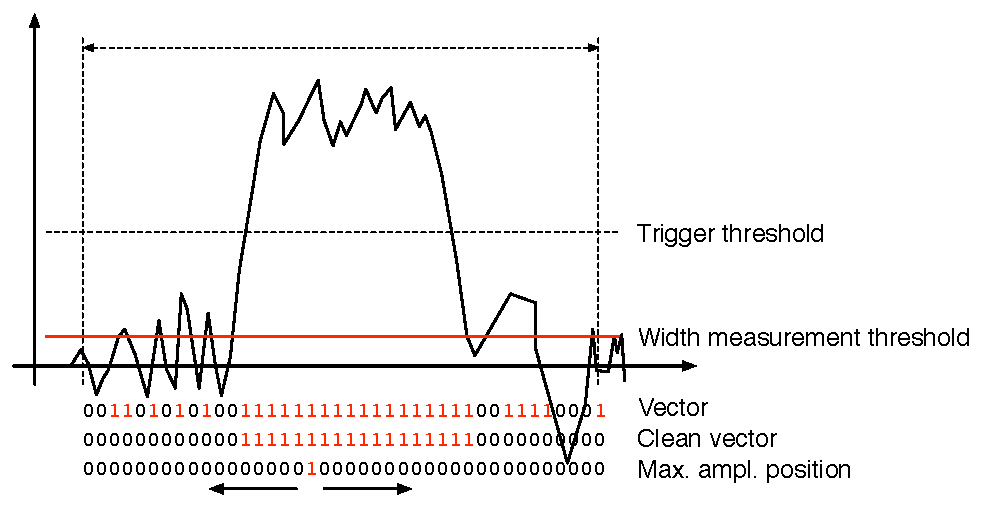
\includegraphics[width=0.7\textwidth]{plots/pulse1}
\caption{A sample pulse. The first vector shows which samples are above the width measurement height. The second vector is a clean vector. The third line shows the position of the maximum amplitude. The vector cleaning algorithm starts from the maximum amplitude and continues in both ways along the vector.}
\label{fig:samplepulse}
\end{figure}

The routine starts from the position of the maximum height. It follows the vector in both ways and finds the first falling edge (0 at this position and 1 at the previous one). From there on it rewrites any binary 1 with a binary 0. The resulting clean vector only has one bunched set of binary ones which are summed, yielding a precise pulse width. The area measurement is similar - it only integrates over the samples marked in the clean vector. Both measurement routines, for area and for width, are implemented separately so that the area routine can have a different threshold set.

This section explains how the algorithm is designed. First, the idea for it was tested using Excel and was only afterwards ported to the VHDL. The underlying algorithm first cleans the vector. Then it passes the cleaned vector either to the width or area measurement. The width measurement module only sums the ones in the vector whereas the area measurement module sums the data samples marked by the cleaned vector. Both modules issue a \emph{valid} signal when they finish the measurement.


 
\subsubsection{Vector cleaning}
This is the most important block. Its inputs are: \emph{vector, parsing active, position of the max. amplitude (PA) and its delay (DA)}. PA is a 32-bit binary number that shows the position of the sample with the maximum amplitude within the data block whereas the DA tells us how many clock cycles after the start of the parsing this PA block is.
\begin{figure}[!ht]
\centering
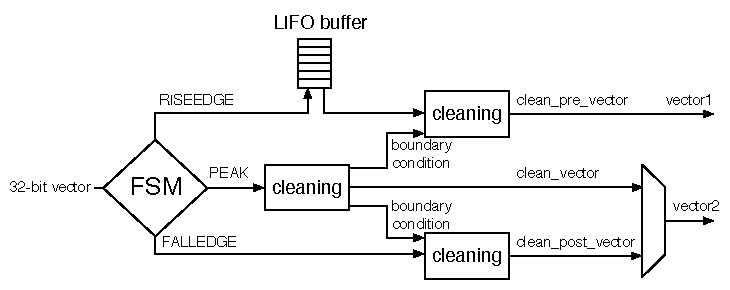
\includegraphics[width=0.7\textwidth]{plots/vector_clean}
\caption{Vector cleaning routine outputs two vectors - one forward in time and one back in time from the peak of the pulse.}
\label{fig:routine}
\end{figure}
The vector cleaning module is designed as a final state machine (FSM) with the states IDLE, RISEEDGE, PEAK, FALLEDGE and READY.  The FSM is idle until it receives the \emph{active} signal from the external module, marking that the vector parsing has commenced. It switches to RISEEDGE, which starts two procedures: 1) it fills the vector of the pulse's rising edge into a last-in-first-out (LIFO) buffer and 2) counts down from the DA value. When this counter reaches 0, the FSM changes its state to PEAK because the current vector on the input is the one containing the maximum amplitude. This data block is sent through the \emph{peak algorithm}, which cleans the vector. The FSM switches to FALLEDGE state. Now both the previously buffered vector of the rising edge and current vector of the falling edge go through the \emph{pre- and post- algorithm} where they are cleaned, but they get their boundary conditions from the \emph{peak algorithm}. The output of this module is therefore two cleaned vectors in parallel -- one forward in time and the other backwards.






\subsubsection{Algorithm}
The underlying algorithm is sequential - it carries out a logic operation on vector bit 0, uses the output of this operation for the operation on bit 1 and so on. This means that it has to carry out 32 logic operations per clock cycle. With each operation taking approximately 0.3~ns, the whole logic chain takes approximately 10~ns to complete. With only 6.4~ns per clock cycle, this means timing errors would occur. To fix the problem, a more complicated \emph{decimated algorithm} was invented. It consists of two parallel logic chains which only take every second bit into account and are at the end merged together. This effectively reduces the number of sequential logic operations to around 18, which is within the timing constraints. 
%Nevertheless, to explain the algorithm, a non-decimated version will be shown first.




\begin{figure}[!ht]
\begin{tabular}{rr}
\subfloat{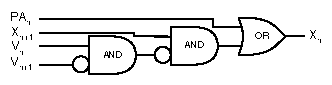
\includegraphics[width=0.47\textwidth]{plots/logic1} \label{fig:logic1}} &
\subfloat{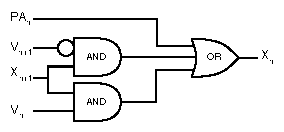
\includegraphics[width=0.47\textwidth]{plots/logic2}  \label{fig:logic2}}
\end{tabular}
\caption{One logic step in the algorithm chain before and after Karnaugh minimisation.}
\end{figure}


\begin{itemize}
\item[Core] This 
\item[Pre]
\item[Post]
\end{itemize}

\subsection{Width measurement}
\begin{figure}[!ht]
\begin{tabular}{rr}
\subfloat{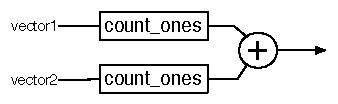
\includegraphics[width=0.27\textwidth]{plots/width_meas} \label{fig:width_meas}} &
\subfloat{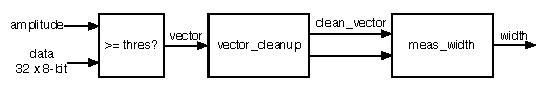
\includegraphics[width=0.67\textwidth]{plots/width}  \label{fig:width}}
\end{tabular}
\caption{This block counts the remaining binary ones in the clean vectors and outputs this value as the pulse width.}
\end{figure}

\subsection{Area measurement}

\begin{figure}[!ht]
\begin{tabular}{rr}
\subfloat{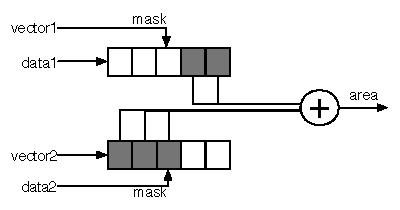
\includegraphics[width=0.30\textwidth]{plots/area_meas} \label{fig:area_meas}} &
\subfloat{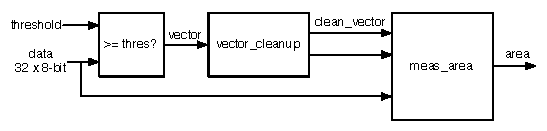
\includegraphics[width=0.64\textwidth]{plots/area}  \label{fig:area}}
\end{tabular}
\caption{This block masks the input data with the clean vector and sums the remaining samples.}
\end{figure}



































\clearpage\clearpage
\subsection{Performance results}
The device has been tested in the lab using a pulse generator as well as several radioactive sources. The results show that: 1) the amplitude, area and width measurement are linear across all input ranges, 2) the highest rate of the PSA algorithm is $\sim10^7$ pulses per second and 3) the lowest SNR where the algorithm still functions is $\sim$5.  

\subsubsection{Rate and linearity}
A pulse generator was used to verify the linearity of the measurements across all input ranges and the highest achievable rate. 
frequency, pulse gen..

\subsubsection{Calibration}
The calibration was done using a \textsuperscript{148}Gd\textsuperscript{239}Pu\textsuperscript{241}Am\textsuperscript{244}Cm source which emits $\upalpha$ particles with four different energies. The PSA in combination with the current amplifier was compared against the 8-bit spectroscopic application in combination with the charge amplifier and a commercial 14-bit spectroscopic readout.

quadruple alpha

\subsubsection{Pulse identification test}
The device was tested using two radioactive sources at the same time. The $^{241}Am$ source of 5.12~MeV $\upalpha$ particles was placed on one side of the diamond. The $^{60}$Co source of photons with the energy o f 1.3~MeV was placed on the other side. The diamond was put in the vacuum chamber to reduce the energy loss of $\upalpha$ particles in the air. The chamber also provided good shielding, reducing the noise pick-up significantly. 
%alpha and cobalt













% ---------------------------------------------------------------------------------------------------------------
\clearpage
\section{Neutron measurements}
\label{sec:nm}
% ---------------------------------------------------------------------------------------------------------------
Semiconductor-based neutron detectors provide a compact technology for neutron detection. However, the cross section of a neutron with the diamond bulk is very low, since it interacts with the core of the atom. Diamond is mainly used to detect charged particles and photons. Hence, a converter foil has to be added to produce second order effects. Incoming neutrons interact with the foil, producing a set of secondary particles and photons. These can then be detected upon hitting the detector bulk. Common neutron interactions that are used in thermal neutron detection are \textsuperscript{10}B(n,$\alpha$)\textsuperscript{7}Li reaction and \textsuperscript{6}Li(n,$\alpha$)\textsuperscript{3}H reaction ($\alpha$ stands for $^4_2$He, see equation~\ref{eq:reaction}). The focus in this chapter will be on the latter of the two. With a foil installed, there are several possibilities for neutrons to interact with the detector system. Each of these interactions ionises the diamond bulk in its own way, resulting in a specific shape of the current pulse. A neutron can: 1) interact with the foil, producing an $\upalpha$ and a \textsuperscript{3}H, 2) interact with a carbon atom, producing an $\upalpha$ and a $\upgamma$ or even three $\upalpha$. The particles in the first case will be produced outside the diamond and will get stopped immediately upon hitting the sensor. The resulting pulses for both particles will have a rectangular shape of the same width, because the carriers will drift with the same speed in both cases. The difference is in the number of free carriers produced - the triton will release more of them, which will in turn induce a higher pulse. 
\begin{equation}
\label{eq:reaction}
   ^6_3Li   +   ^1_0n \;\rightarrow\; ^3_1H_{(2.73 MeV)} + \alpha_{(2.05 MeV)}
\end{equation}

It turns out that neutron reactors emit large amounts of $\upgamma$ radiation in energy range up to 3~MeV. This already affects measurements of $\upalpha$ particles, the energy of which peaks at 2.05 MeV in the case of \textsuperscript{6}Li converter foil. However, $\upgamma$ background radiation could be suppressed by discriminating current pulses of photons and $\alpha$ particles. This idea has already been implemented in offline analysis. The results show that the background photons can be subtracted successfully. In order to improve the speed of the readout system and pulse analysis, the algorithm has been ported to FPGA where it discriminates particles in real time. 


\subsection{Thermal neutron spectroscopy}
ROSY readout device with the implemented Pulse Shape Analysis was put to a test at Atominstitut in Vienna. Their TRIGA2 neutron reactor is capable of delivering thermal neutrons with the energy 0.012~eV at a rate of 1000~neutrons cm$^{-2}$ $s^{-1}$, however with a considerable $\gamma$ background. 

With the measurement setup already commissioned, the experiment started delivering data almost immediately. First, the device was calibrated using an unsealed monochromatic $\alpha$-source with the energy $E_\alpha=5.12MeV$. Then the diamond detector was exposed to the beam. Secondary reaction products ($\alpha$ and \textsuperscript{3}H particles), created by neutrons hitting the converter foil, were detected by the diamond sensor, together with a significant photon background. Then the pulse identification algorithm was applied to discriminate between the reaction products and the photons.

\subsubsection{Measurement setup}
%The diagram in figure~\ref{fig:rochain} shows the readout chain of the measurement system, which consists of a detector assembly, a signal preamplifier, a readout device and a controller PC. 
The main parts of the detector were an scCVD diamond sensor sized $4.7\times4.7$~cm$^2$ and a $1.8~\upmu$m thick LiF converter foil, both embedded in an RF-tight PCB. The diamond sensor was biased with high voltage and capacitively coupled to CIVIDEC's C2 40~dB wide bandwidth signal preamplifier. A 5~m long BNC cable connected the preamplifier to CIVIDEC ROSY box. The detector assembly together with the preamplifier was fixed in front of an exit hole of the reactor.



\subsubsection{Results}





% ---------------------------- comment out when compiling the full document -------------------
\end{document}
% ---------------------------------------------------------------------------------------------------------------
